% Chapter on Online Monitoring, Data Quality Monitoring & Event Displays
% 10 pages

\graphicspath{{OnlineMonitoring/Figs/}}

%----------------------------------------------------------------------------------------------------------------------------------------------------------------------------
\chapter{Online Monitoring and Event Displays for the 35~ton Experiment}\label{chap:OnlineMonitoring}

Monitoring of the data collected during the running of an experiment is imperative to ensure a high quality is maintained.  Such monitoring is often provided in real-time (`online monitoring'), summarising the data from the current run, or in near real-time (`nearline monitoring'), summarising data over runs from typically the previous day, week or month to represent the longer term fluctuations in the data quality.  An event display, designed to illustrate physics events as they occur in the detector, is another desirable feature that is particularly useful during data collection.  The system developed to provide online feedback, including a basic event display, for the 35~ton Phase~II data taking period is the subject of this present chapter.

The framework was designed to be flexible and provide prompt feedback for those operating the experiment; it was thus included as part of the DAQ system, discussed in Section~\ref{sec:35tonDAQ}.  The monitoring framework itself is the subject of Section~\ref{sec:OnlineMonitoring}, with its two functions, data quality monitoring and producing online event displays, presented in Sections~\ref{sec:DQM} and~\ref{sec:EventDisplay} respectively.  Finally, the web interface developed to allow synchronisation of this monitoring data to a dedicated web page for ease of access is briefly described in Section~\ref{sec:WebInterface}.

% Moved to 35ton chapter
%% %----------------------------------------------------------------------------------------------------------------------------------------------------------------------------
%% \section{The DAQ Framework}\label{sec:lbne-artdaq}

%% Experiments at FNAL are migrating to \textit{artdaq}, a centrally-maintained data acquisition system built on the art framework utilised by all offline software written for experiments hosted at the lab.  The DUNE 35~ton experiment was one of the first to use this new software (only LArIAT had previously used it for data taking) and used an experiment specific system named lbne-artdaq.
%% %% \footnote{Since the formation of the DUNE experiment occurred only a few months before the running of the 35~ton, all online software maintained the use of the outdated `lbne' descriptor to prevent unnecessary potential problems associated with large scale code changes and alleviate the risk of further delays.  It should be again stressed that the 35~ton was recognised by the DUNE collaboration as an integral part of the DUNE plan and the use of \textit{lbne} was in no way an indication of a project associated only with the dissolved previous experiment!}.
%% A general overview of lbne-artdaq is shown in Figure~\ref{fig:lbne-artdaq}.

%% %% \begin{figure}
%% %% \centering
%% %%   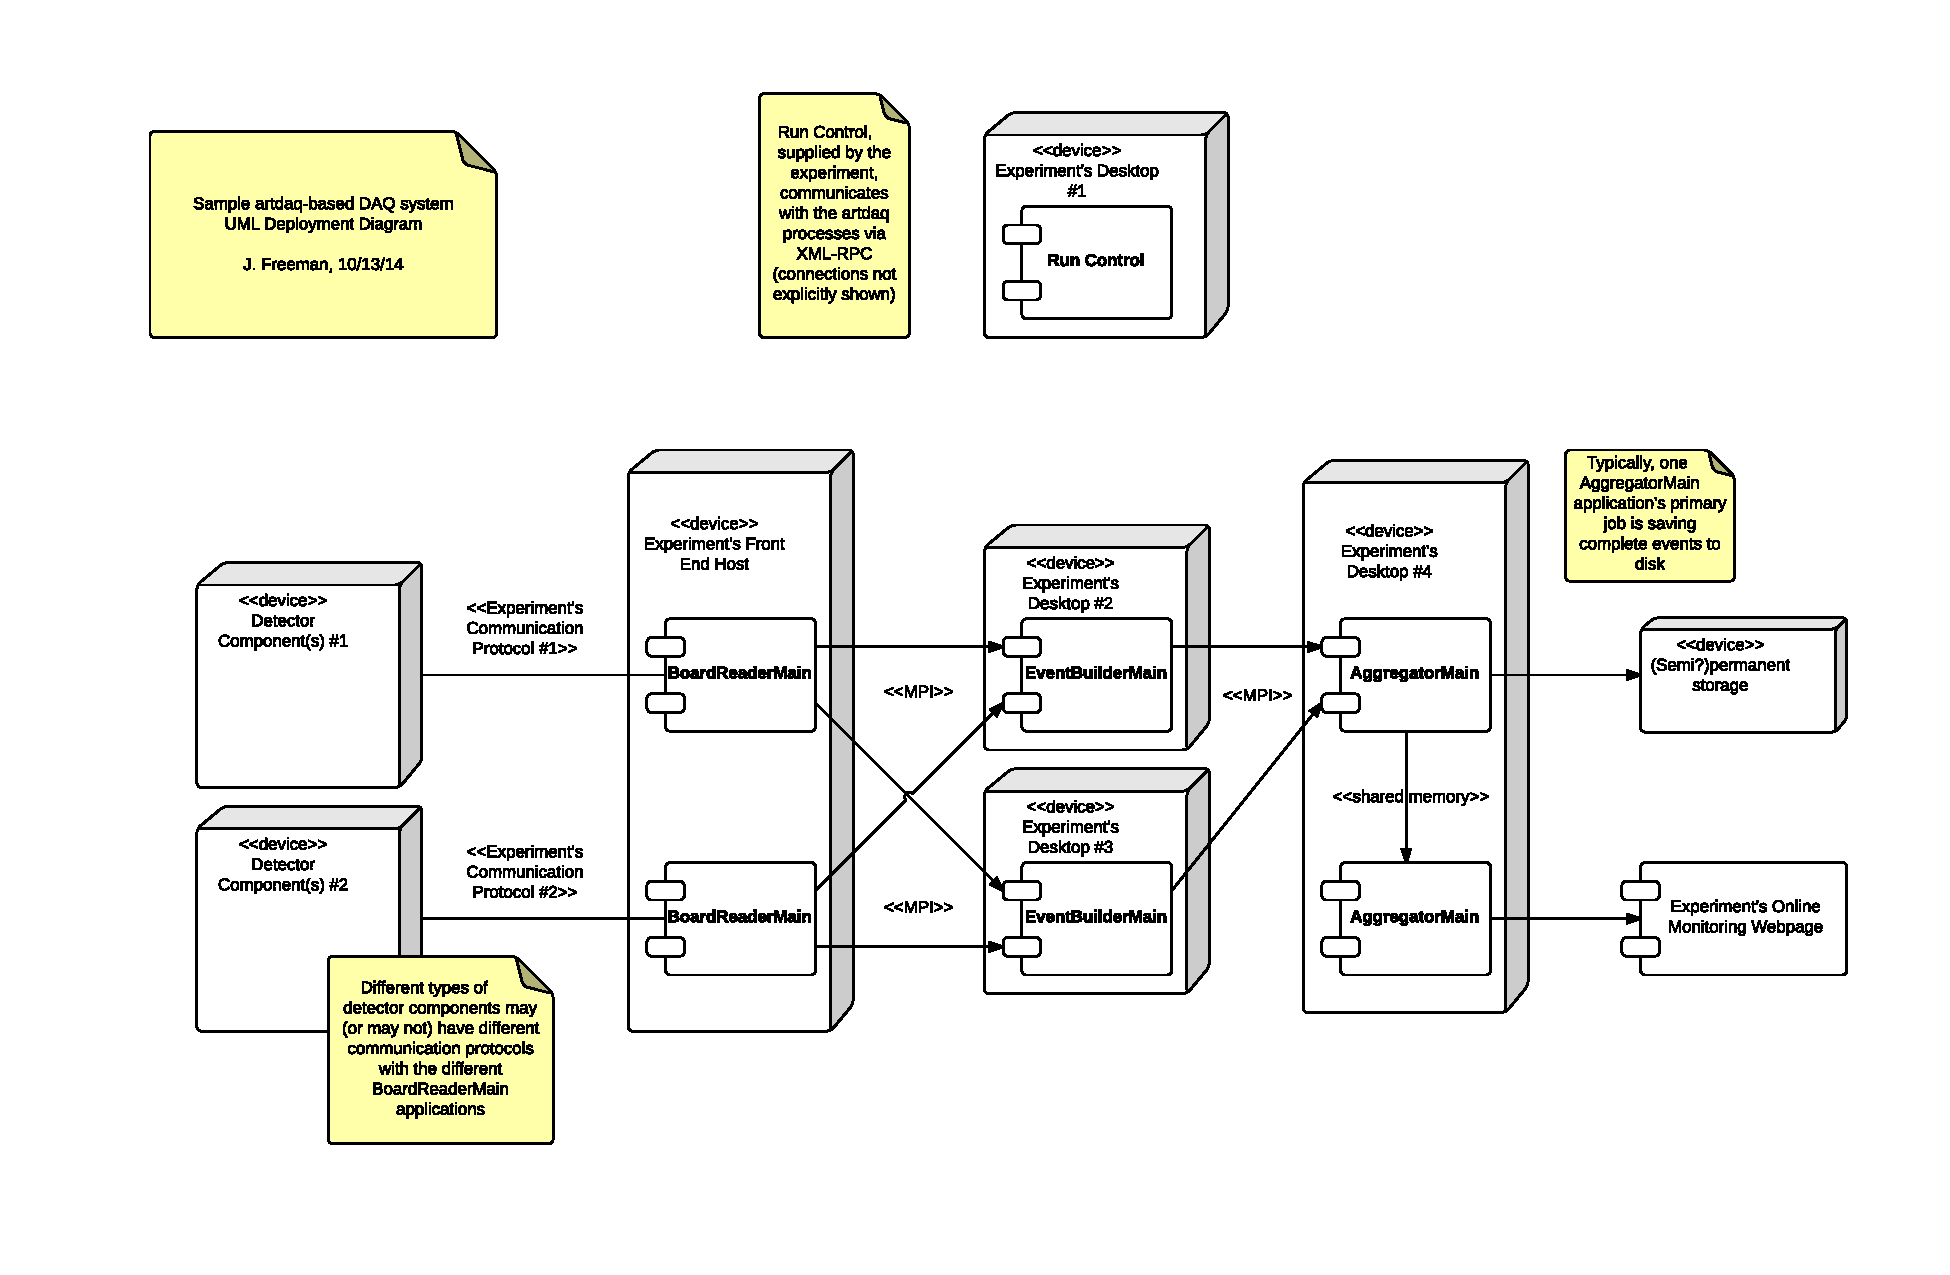
\includegraphics[width=16cm]{artdaqFramework.pdf}
%% %%   \caption[The \textit{lbne-artdaq} framework]{Overview of the \textit{lbne-artdaq} framework used for data acquisition by the DUNE 35~ton experiment \cite{Freeman2014}.  See the text for a complete description.}
%% %%   \label{fig:lbne-artdaq}
%% %% \end{figure}

%% Data flows from left to right and pass through components common to most DAQ systems.  Closest to the detector components (i.e. the RCEs, SSPs and PTB [see Section~\ref{sec:DetectorComponents}]) are the board readers which take the output from the firmware as soon as it is ready and sends it downstream to the event builders.  There exists a board reader for each of the detector components (totalling 24) and each is unaware of the existence of the others.  It is the job of the event builders to assemble a full `event' from these individual `fragments' passed on from each of the detector elements.  An event is complete once composed of a full set of fragments and the event builders will wait to receive them all before sending the data onwards to the aggregators.

%% There are two aggregators which take the full events but process them in very different ways.  All the data passes through only the first aggregator, whose function it is to write the output to disk and thus end processing by the DAQ.  The second aggregator receives no events but instead has access to the shared memory occupied by the data as it passes through the first aggregator; it is thus designed specifically for the purpose of monitoring and in no way affects the data or the output from the first aggregator.  It is within this second aggregator process that the online monitoring system described in the proceeding section is designed to run.

%% Each of the DAQ processes runs on a machine on the private DAQ network and is configured as normal within art (using the \textit{fhicl} (Fermilab Hierarchical Configuration Language) configuration language).  Two nodes on the main FNAL network (lbne-gateway01/02) provide access to these private machines, of which there are 7 (lbnedaq1-7), and contain all scripts and setup necessary to run through the DAQ via a command line interface.

%----------------------------------------------------------------------------------------------------------------------------------------------------------------------------
\section{The Online Monitoring Framework}\label{sec:OnlineMonitoring}

The framework developed for the monitoring system had the following design goals:
\begin{itemize}
\item to be able to analyse the data read out of memory in its raw `DAQ format';
\item to be computationally efficient to allow for processing at the event rate (data taking rate);
\item to provide the flexibility for further monitoring plots to be added with ease;
\item to allow for use of an online event display to provide comprehensible images of the raw data.
\end{itemize}
In general, the developed system succeeded in all these goals and provided invaluable information, becoming an integral tool in the commissioning and the data taking during the 35~ton Phase~II run.  An illustration of the framework is shown in Figure~\ref{fig:OnlineMonitoringFramework}.

\begin{figure}
  \centering
  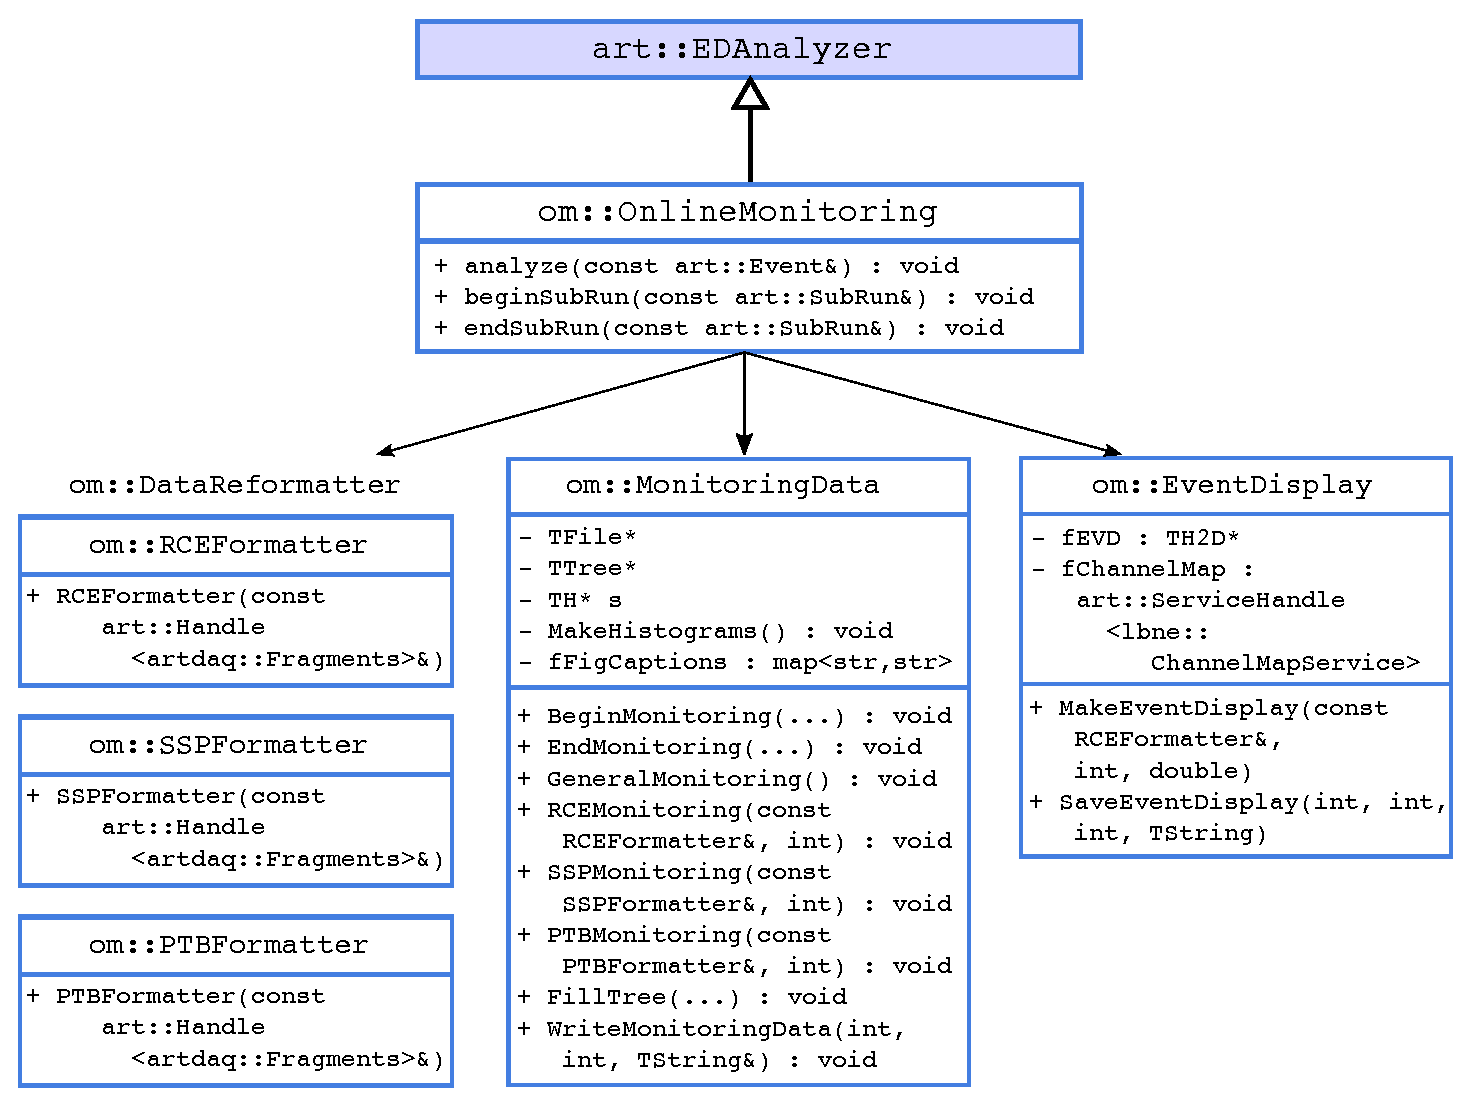
\includegraphics[width=12cm]{softwareFramework.eps}
  \caption[The software framework designed and built for online monitoring during the 35~ton Phase~II run.]{The software framework designed and built for online monitoring during the 35~ton Phase~II run.}
  \label{fig:OnlineMonitoringFramework}
\end{figure}

%----------------------------------------------------------------------------------------------------------------------------------------------------------------------------
\subsection{Design of the Monitoring Framework}\label{sec:MonitoringFrameworkDesign}

The setup consists of a central `module', \texttt{OnlineMonitoring\_module.cc}, which is configured within the \textit{art} framework through its base class.  The OnlineMonitoring class manages the running of the system and owns instances of further classes each designed for a specific purpose, controlling the data flow by calling the relevant methods when required.  Once an event has been obtained, the data for each component is processed and repackaged into RCEFormatter, SSPFormatter and PTBFormatter objects.  The purposes of this method are
\begin{itemize}
\item to provide an interface between the raw data and the methods which analyse the data.  This is important as it provides a single point of maintenance for when formats change and allow for various `DAQ modes' to use the same analysis code;
\item to separate interaction with the DAQ from the handling of output data objects;
\item to facilitate random access of the data for more detailed analysis which would not be possible if just processing linearly.
\end{itemize}
The main drawback to performing this step is it requires all the data to be held in memory until the end of the event and represents basically the same information as initially present.  However, it was decided the advantages were worth the required compromises in memory usage and no problems were apparent during the course of the run except when operating at the very limits of DAQ capabilities.

These reformatted data objects are then passed to the methods in the MonitoringData class for analysis.  This class owns all of the data products which are output from the monitoring (e.g. histograms, graphs, trees and files) and deals with their filling and writing out when required.  This is discussed further in Section~\ref{sec:DQM}.

The event display is handled by its own dedicated class, EventDisplay, which has methods for making the displays and saving them as an image in the correct place when required.  It is designed to accept the reformatted RCE object and presents the data in as meaningful a way as possible; this is detailed fully in Section~\ref{sec:EventDisplay}.

%----------------------------------------------------------------------------------------------------------------------------------------------------------------------------
\subsection{Interface with the DAQ Framework}

The 35~ton DAQ, previously discussed in Section~\ref{sec:35tonDAQ}, was based on the \textit{lbne-artdaq} framework illustrated in Figure~\ref{fig:lbne-artdaq}.  This system has support for running online monitoring embedded into its design philosophy, with the Aggregator2 process allowed to access data from shared memory as it is managed by Aggregator1.  The controlling monitoring module, discussed in Section~\ref{sec:MonitoringFrameworkDesign}, may be configured to run within this second aggregator process and thus receive events in real-time as they pass through the data acquisition system.

The events are passed to the Aggregator2 process by the framework when resources are available; if this is not possible then the event is simply skipped.  This behaviour does not affect the processing of the data through Aggregator1 and the events missed by the monitoring will still be saved to disk.  The issues arise primarily when the monitoring runs slower than the data taking rate (i.e. when producing monitoring information for an event takes longer than the length of the event itself) and were largely inevitable due to the number of required plots and the computational resources necessary for tasks such as FFTs and event displays.  As most monitoring plots, such as TPC noise, require only a few events, they are mostly unaffected; however, there are implications when calculating rates and similar quantities.  During normal running, as many as half of the events may be missed by the monitoring, depending on the detail of the plots being produced.  Using multiple threads detached from the main processes was considered, particularly when making events displays, as way to increase the event exposure but, due to the potential computing issues which may arise, it was decided not to implement this for the purposes of a short prototype run.

Each of the DAQ processes run on a machine on the private DAQ network and are configured as normal within \textit{art}, using \textit{fhicl}.  Two nodes on the main FNAL network (lbne-gateway01/02) provide access to these private machines, of which there are 7 (lbnedaq1-7), and contain all scripts necessary to setup, configure and run the DAQ via a command line interface.

%----------------------------------------------------------------------------------------------------------------------------------------------------------------------------
\subsection{Writing the Monitoring Data}\label{sec:WritingMonitoringData}

The data objects are newly created for each subrun and are written out at three points during data taking:
\begin{itemize}
\item an initial write out N seconds after the start of the subrun;
\item at frequent intervals during the subrun, every M seconds;
\item at the end of the subrun.
\end{itemize}
The parameters N and M are configurable and were set to 30 and 500 respectively for normal data taking.  The data products are only cleared at the end of a subrun, so any intermediate writing out of data simply refreshes the current plots.

The event displays are computationally expensive to make and so were only created once per subrun during normal running.  However, since a subrun was automatically stopped, and a new one started, by the DAQ once the output file had reached 5~GB in size, and (since zero suppression was not utilised at any point during the run) this occurred on average every four minutes, a new event display was made relatively frequently.

All the output data were saved on a shared disk on the gateway DAQ machines for further use.  This is discussed in Section~\ref{sec:WebInterface} below.

%----------------------------------------------------------------------------------------------------------------------------------------------------------------------------
%% \subsection{Configuring the Monitoring}\label{sec:MonitoringConfiguration}

%% [Possibly don't need this section...]
%% The system was designed to be flexible and many parameters were available to control the running of the monitoring.  These are listed and described below, with default parameter provided in brackets.

%% \begin{itemize}
%% \item TPCModuleLabel (``daq'') -- art module label for TPC data saved in the DAQ;
%% \item PhotonModuleLabel ([ ``sparseSsp'', ``daq'' ]) -- art module label for photon data saved in the DAQ;
%% \item TriggerModuleLabel (``daq'') -- art module label for counter data saved in the DAQ;
%% \item DetailedMonitoring (false) -- fills more, and usually more computationally expensive, data;
%% \item ScopeMonitoring (false) -- support for a different DAQ running mode, `scope mode';
%% \item DataDirPath (``/storage/data/'') -- path at which the data files are saved by the first aggregator;
%% \item MonitorSavePath (``/data2/lbnedaq/monitoring/'') -- location to save DQM data;
%% \item EVDSavePath (``/data2/lbnedaq/eventDisplay/'') -- location to save event displays;
%% \item PedestalFile (``/data2/lbnedaq/pedestal.csv'') -- location of the most recent pedestal file, containing pedestals for all channels.  This was used for pedestal subtraction when making event displays;
%% \item ImageType (``.png'') -- the format to save any images;
%% \item MonitoringRefreshRate (500) -- how often to write out the most recent monitoring data plots;
%% \item InitialMonitoringUpdate (30) -- how long after starting a new subrun to initially write out the data;
%% \item EventDisplayRefreshRate (60) -- how often to refresh the event display when not just making one per subrun;
%% \item LessFrequentFillRate (20) -- how often to fill the more computationally expensive plots;
%% \item DriftVelocity (0.9 \#mm/us) -- rough drift electron velocity, used for calculating the x coordinate for the event display;
%% \item CollectionPedestal (550) -- the default pedestal value if the file isn't readable;
%% \item MicroslicePreBuffer (5) -- how many microslices are saved by the RCEs before the one containing the trigger;
%% \item MicrosliceTriggerLength (5) -- the length of the trigger.
%% \end{itemize}

%----------------------------------------------------------------------------------------------------------------------------------------------------------------------------
\section{Data Quality Monitoring}\label{sec:DQM}

The overarching aim of the online monitoring system was to provide direct feedback to the experimental operators with information about the status of the data taking and the quality of the data.  This is vital for various different aspects of data taking, for example
\begin{itemize}
\item ensuring all detector components being used in the current run are receiving and processing data;
\item noting the TPC readout has entered the `high noise state' and acting accordingly;
\item checking the trigger rates from the external cosmic muon counters are feasible.
\end{itemize}

The monitoring was diagonalised in a similar way to the DAQ readout with data from the TPC, photon detector and external counters processed separately.

%----------------------------------------------------------------------------------------------------------------------------------------------------------------------------
\subsection{TPC Monitoring}\label{sec:TPCMonitoring}

Monitoring of the TPC data involved mainly considering various distributions of the ADC values provided by the front-end boards, separated by channel, board and APA.  The mean and RMS of the ADC values for a given channel provides information such as the measured pedestal and the level of noise being read out.  The uncorrelated component of the noise can be monitored using the concept of `DNoise'; this considers the difference in ADC value between two neighbouring channels at a given readout time and represents the level of noise which would be impossible to remove by the use of coherent noise filters only.  Unfortunately, for the 35~ton, this uncorrelated component made up most of the noise across all channels (see Figure~\ref{fig:DQMPlot1}).  FFTs of the signal waveforms, performed separately for each RCE, were also useful in monitoring bands of noise in frequency space.

Monitoring of various other problems, such as the digitiser stuck code issue, synchronisation concerns resulting in a different number of microslices being saved in corresponding RCE millislices, and the asymmetry of bipolar pulses, were added as these issues became apparent during the commissioning.

%----------------------------------------------------------------------------------------------------------------------------------------------------------------------------
\subsection{Photon Detector Monitoring}\label{sec:PhotonMonitoring}

Analogously to the TPC data, monitoring of the photon detectors mainly involved considering various ADC distributions separated by optical channel and by photon detector.  The peak height, pedestal and integral of each waveform were also considered as a function of channel to ensure each were operating consistently.

The triggers sent on by the SSPs were also studied; unfortunately, due to the design of the monitoring framework (with it not guaranteed to receive each event), trigger rates were challenging to compute.  It was decided to leave them in the monitoring but only consider the relative rates; the monitoring code may be utilised offline, processing closed files on disk, to determine accurate rates by ensuring all events are considered.  Along with the trigger rate, the number of triggers, the fraction of events containing a trigger and the number of readout ticks within each trigger were also considered.

During installation, one photon detector was erroneously left unconnected to its SSP and so was unavailable during the run.  This was discovered using the online monitoring framework but unfortunately only following the completion of the installation and the sealing of the cryostat.

%----------------------------------------------------------------------------------------------------------------------------------------------------------------------------
\subsection{External Counter Monitoring}\label{sec:CounterMonitoring}

Since monitoring the external counters primarily involves considering trigger rates, a similar issue to the photon detector monitoring was encountered; as with the SSP triggers, the rates were only considered relative to different counters.  For each counter, the hit rate and the average activation time were monitored to ensure counters in similar positions were recording comparable cosmic muon data.  The number and type of payloads sent on from the PTB were also detailed so the amount of data, along with information about what the data are comprised of, could be monitored.

%----------------------------------------------------------------------------------------------------------------------------------------------------------------------------
\subsection{General Monitoring}\label{sec:GeneralMonitoring}

A variety of useful quantities not pertaining to any specific subcomponent were also monitored to assure smooth data taking.  These include the size of output files and the average event size from recent runs, information about which detector subcomponents are taking data and the number of events seen by each, and also synchronisation information between various detector components.

%----------------------------------------------------------------------------------------------------------------------------------------------------------------------------
\subsection{DQM Plots}\label{sec:DQMPlots}

The DQM component of the online monitoring produced around 60 figures for each subrun, illustrating the data discussed in Sections~\ref{sec:TPCMonitoring},~to~\ref{sec:GeneralMonitoring}.  A sample subset of these figures is shown in Figure~\ref{fig:DQMPlots}.
%; refer to Appendix \# for a reproduction of all figures from a particular run. {\color{red} Lee: I'm not sure this appendix is necessary, but happy to add it if you think it would be good.  Beware it would just be $\sim$60 plots!}

\begin{figure}
  \centering
  \begin{subfigure}[t]{0.48\linewidth}
    \centering
    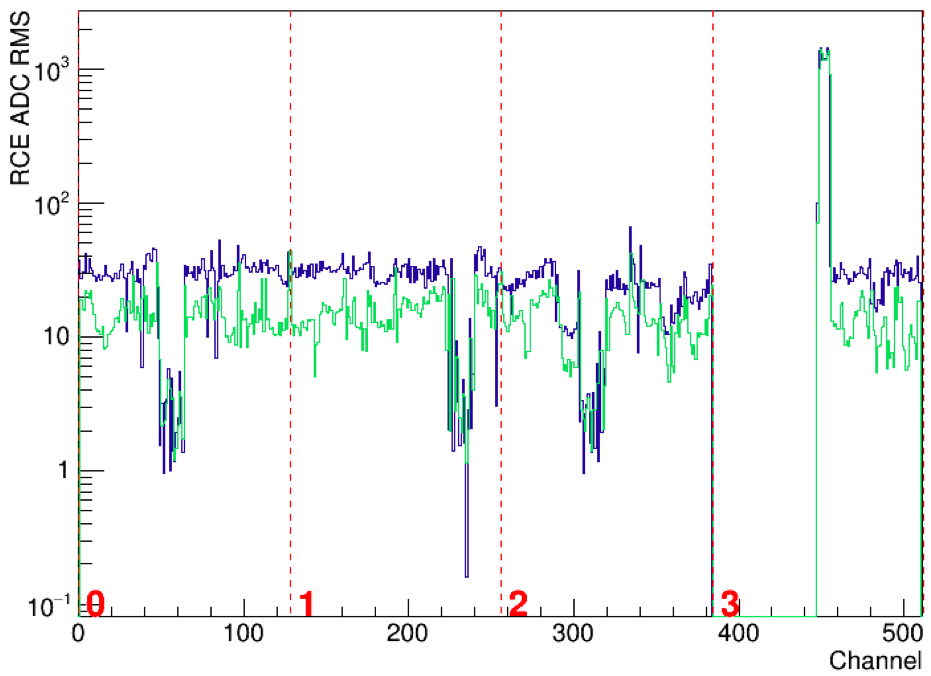
\includegraphics[width=0.95\textwidth]{DQM1.png}
    \caption{TPC noise.}
    \label{fig:DQMPlot1}
  \end{subfigure}
  \begin{subfigure}[t]{0.48\linewidth}
    \centering
    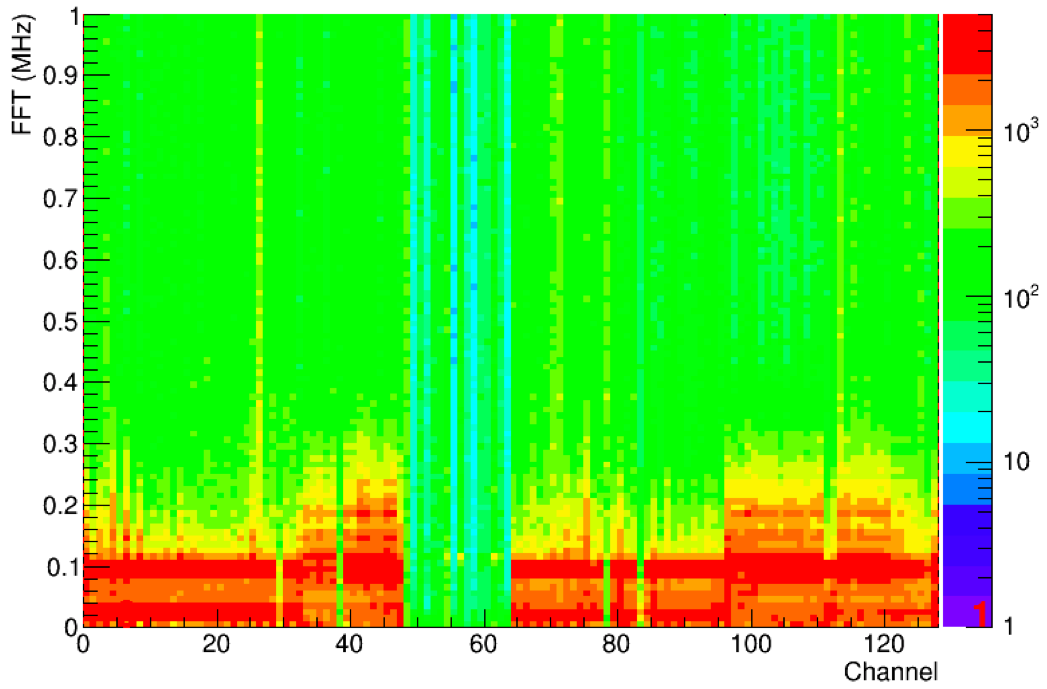
\includegraphics[width=0.95\textwidth]{DQM2.png}
    \caption{FFT.}
    \label{fig:DQMPlot2}
  \end{subfigure}
  \begin{subfigure}[t]{0.48\linewidth}
    \centering
    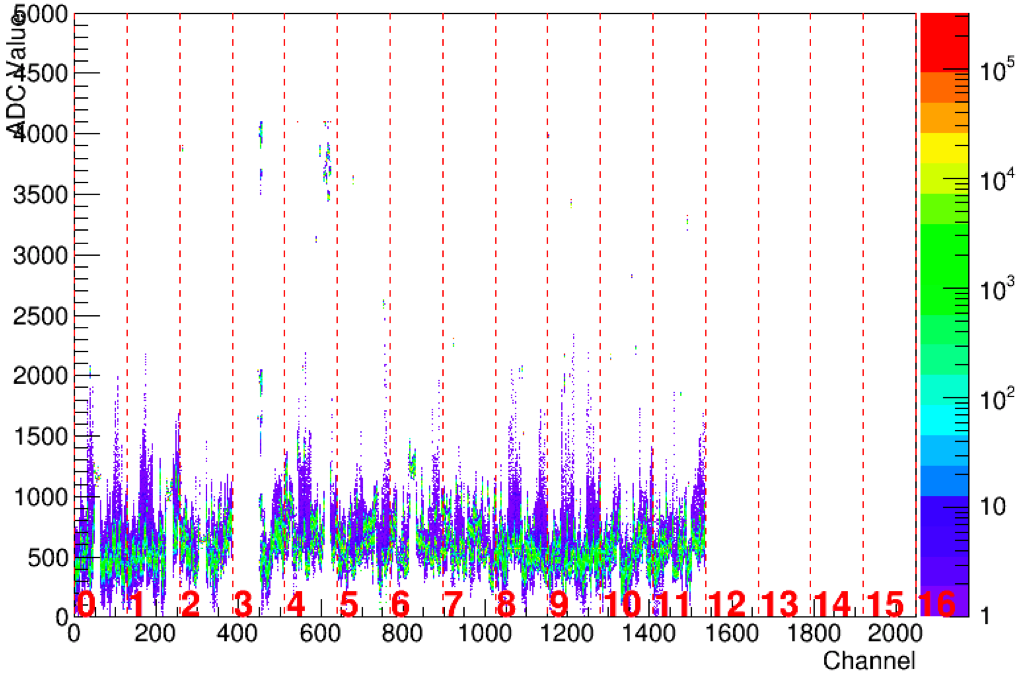
\includegraphics[width=0.95\textwidth]{DQM3.png}
    \caption{ADC values as a function of channel.}
    \label{fig:DQMPlot3}
  \end{subfigure}
  \begin{subfigure}[t]{0.48\linewidth}
    \centering
    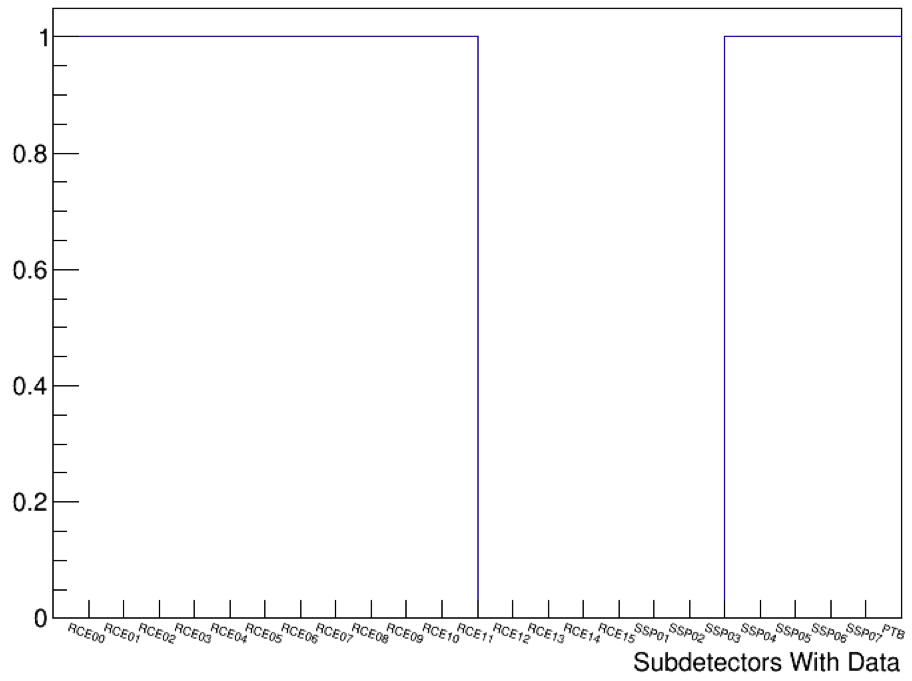
\includegraphics[width=0.95\textwidth]{DQM4.png}
    \caption{Subdetectors which are successfully collecting data.}
    \label{fig:DQMPlot4}
  \end{subfigure}
  \caption[Selection of figures made by the Data Quality Monitoring framework during 35~ton Phase~II running.]{Selection of figures made by the Data Quality Monitoring framework during 35~ton Phase~II running.  Figure~\ref{fig:DQMPlot1} shows the TPC noise; the total noise (RMS of the ADC values) is shown in blue and the uncorrelated component of this noise in green.  The FFT of a waveform read out by the first RCE (channels~1--128) is shown in Figure~\ref{fig:DQMPlot2} and a 2D plot showing the ADC values for each channel, hugely useful as it demonstrates both the mean and RMS for all channels together, is depicted in Figure~\ref{fig:DQMPlot3}.  Figure~\ref{fig:DQMPlot4} shows the subdetectors which are successfully collecting data and may be used to note one quarter of the TPC readout, along with three photon detector readouts, were turned off in this subrun.}
  \label{fig:DQMPlots}
\end{figure}

%----------------------------------------------------------------------------------------------------------------------------------------------------------------------------
\section{Online Event Display}\label{sec:EventDisplay}

One of the highlights of being in ROC West (Remote Operation Control room at FNAL) during data taking was watching the online event display refresh with updated images representing cosmics passing through the detector.  In addition to the interesting visual display of interactions in the detector, it allowed for data to be monitored with ease; high noise states, poor LAr purity and drift field problems were all immediately evident from the display.

Given the structure of the data when read out of the detector, it proved challenging finding a comprehensible way to represent events.  The construction of such a display is the subject of this section.

%----------------------------------------------------------------------------------------------------------------------------------------------------------------------------
\subsection{Selecting the Data}\label{sec:SelectingEVDData}

The raw data formats for the various 35~ton data streams were discussed in detail in Section~\ref{sec:35tonDataFormats}.  Each DAQ event comprises a collection of millislices, one for each of the detector subsystems (RCEs, SSPs, PTB), with further structure specific to each system and comprehensively illustrated in Figure~\ref{fig:35tonDataFormat}.  An example triggered event in the 35~ton data is demonstrated in Figure~\ref{fig:35tonTriggeredEvent}.

Since the event display runs online, a suitable selection must be applied to ensure the full physics event occurs within the current DAQ event; proceeding and preceding events are inaccessible during running.  This is achieved by noting whether or not a trigger occurred (i.e. microslices contain nanoslices), and in which microslice it occurred, when reformatting the RCE data in DataReformatter.  For the event display, an event is only useful if the trigger occurred within a certain range (e.g. Microslice~5 to Microslice~10), ensuring all the filled microslices are present within the current millislice.  The event display is then filled for a given range of microslices around the trigger to capture all the physics data.

%----------------------------------------------------------------------------------------------------------------------------------------------------------------------------
\subsection{Representing the Data}\label{RepresentingEVDData}

The wrapped nature of the induction wires, and the inability to perform disambiguation without full reconstruction, results in only data from the collection plane being useful for an online event display.  Use of a second dimension is possible if the detector is viewed from above and by using the drift time as a coordinate.  This necessitates the two centre APAs be shown together as one combined readout structure and a global two-dimensional coordinate system established for the entire detector.  The wire coordinate is defined simply by counting wires from the collection planes across all APAs and incorporating fake wires between the frames, and the time coordinate may be used to take multiple drift regions into account by correcting all charge deposited in the short drift region to negative ticks.

The event displays are filled with the raw ADC values provided by the FE readout without the use of reconstruction.  An approximate pedestal subtraction is possible by working with the system used to record these pedestal values.  During data taking, the shifter would perform a run at least once per shift to produce a file containing all the calculated pedestals on each channel for subsequent uploading to a database for offline use.  By ensuring a copy of the most recent file is always available to the monitoring framework, the pedestals may be corrected for and the charge represented as accurately as possible.  To limit noisy channels and to correct for accidental negative charge, the pedestal-subtracted ADC values are only included if within the range $0-250$.  Finally, given the relatively low signal-to-noise ratio, it was decided a grey-scale image showed the best resolution for observing tracks in the cryostat.

An example event display is shown in Figure~\ref{fig:EVD}.

\begin{figure}
  \centering
  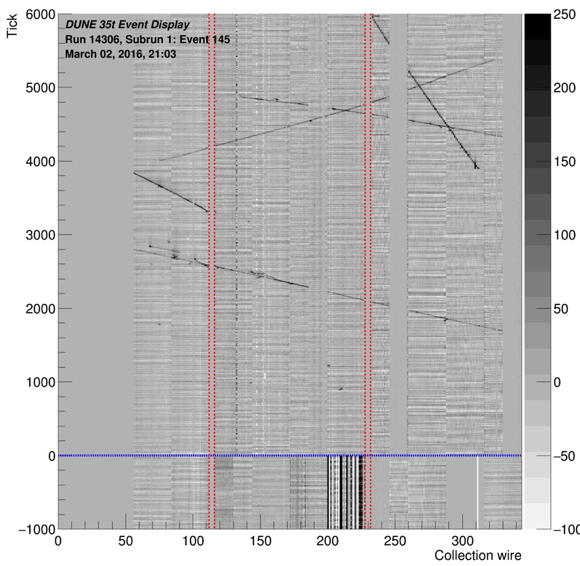
\includegraphics[width=14cm]{evd.png}
  \caption[Example online event display made by the Online Monitoring framework.]{Example online event display made as part of the online monitoring framework for run 14306 (2nd March, 2016).  The view is from the top of the detector looking down; the red lines represent the spaces between the APAs and the blue line the location of the APA frames, separating the long and short drift regions.}
  \label{fig:EVD}
\end{figure}

%----------------------------------------------------------------------------------------------------------------------------------------------------------------------------
\section{Monitoring Web Interface}\label{sec:WebInterface}

The output of the monitoring is vital in assuring the experiment continues to take high quality, analysable data.  To facilitate this process, a web interface was developed to enable all useful information to be displayed and accessed in a convenient, universal location.  This interface, along with the complementary web page, was relatively basic but was functional and performed all that was required for the purposes of a short prototype run.  The method of automating the transfer of the monitoring data from where it was saved by the DAQ process to somewhere accessible by the web server is briefly described in Section~\ref{sec:AutomatedDataTransfer} and the web page itself is overviewed in Section~\ref{sec:WebPage}.

%----------------------------------------------------------------------------------------------------------------------------------------------------------------------------
\subsection{Automated Data Transfer}\label{sec:AutomatedDataTransfer}

Ensuring the monitoring output was available in the correct place when needed was the most complicated part of the web interface.  This was achieved using a combination of disk mounting and automated scripts, demonstrated in Figure~\ref{fig:WebInterface}.

\begin{figure}
  \centering
  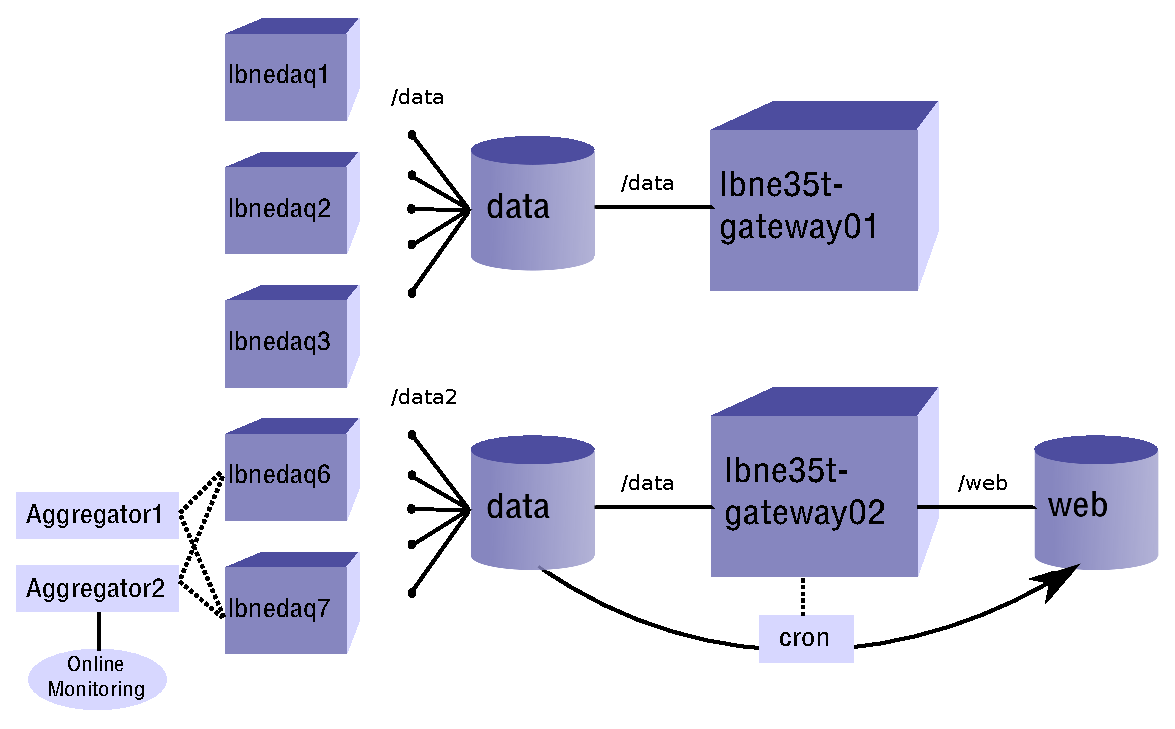
\includegraphics[width=12cm]{webInterface.eps}
  \caption[Schematic showing the interface between the online monitoring system and the web.]{Schematic showing the interface between the online monitoring system and the web.  The DAQ machines are shown as rectangles with their disks represented as cylinders.  Connections between a node and a disk are shown as straight lines, with dotted lines representing processes running on the machine.}
  \label{fig:WebInterface}
\end{figure}

The DAQ aggregator processes run on the lbnedaq6 and lbnedaq7 nodes, requiring any saved output be placed in a location accessible to these machines.  Mounting a disk belonging to a gateway node onto these private machines and saving the output directly onto this ensured the data may be available outside of the private network.  The constraints placed on the configuration by the DAQ group, which preferred nothing other than DAQ processes to run on lbne35t-gateway01, required a second gateway node, lbne35t-gateway02, be utilised.  The web transfer framework was completed by mounting the Fermilab web area onto this machine and utilising an automated job to copy the monitoring data from the disk to the relevant part of the web server.  The frequency of this job, 30 seconds, defined the maximum latency one could expect between data being written out and images appearing online.

%----------------------------------------------------------------------------------------------------------------------------------------------------------------------------
\subsection{Web Page}\label{sec:WebPage}

The web page was hosted at FNAL and located at lbne-dqm.fnal.gov.  When the monitoring framework initiates a write out of all data products, the HTML necessary to correctly display these images is also written and saved as part of the output.  This is copied, along with all the images and data files, to the web area as discussed in Section~\ref{sec:AutomatedDataTransfer}.  The web page was basic but fulfilled all fundamental requirements for 35~ton monitoring; it had dedicated pages for all the data quality monitoring information and the online event display (the nearline monitoring was also hosted at this website but is not described here).  See Figure~\ref{fig:WebPage} for a demonstration of web page and example navigation.

\begin{figure}
  \centering
  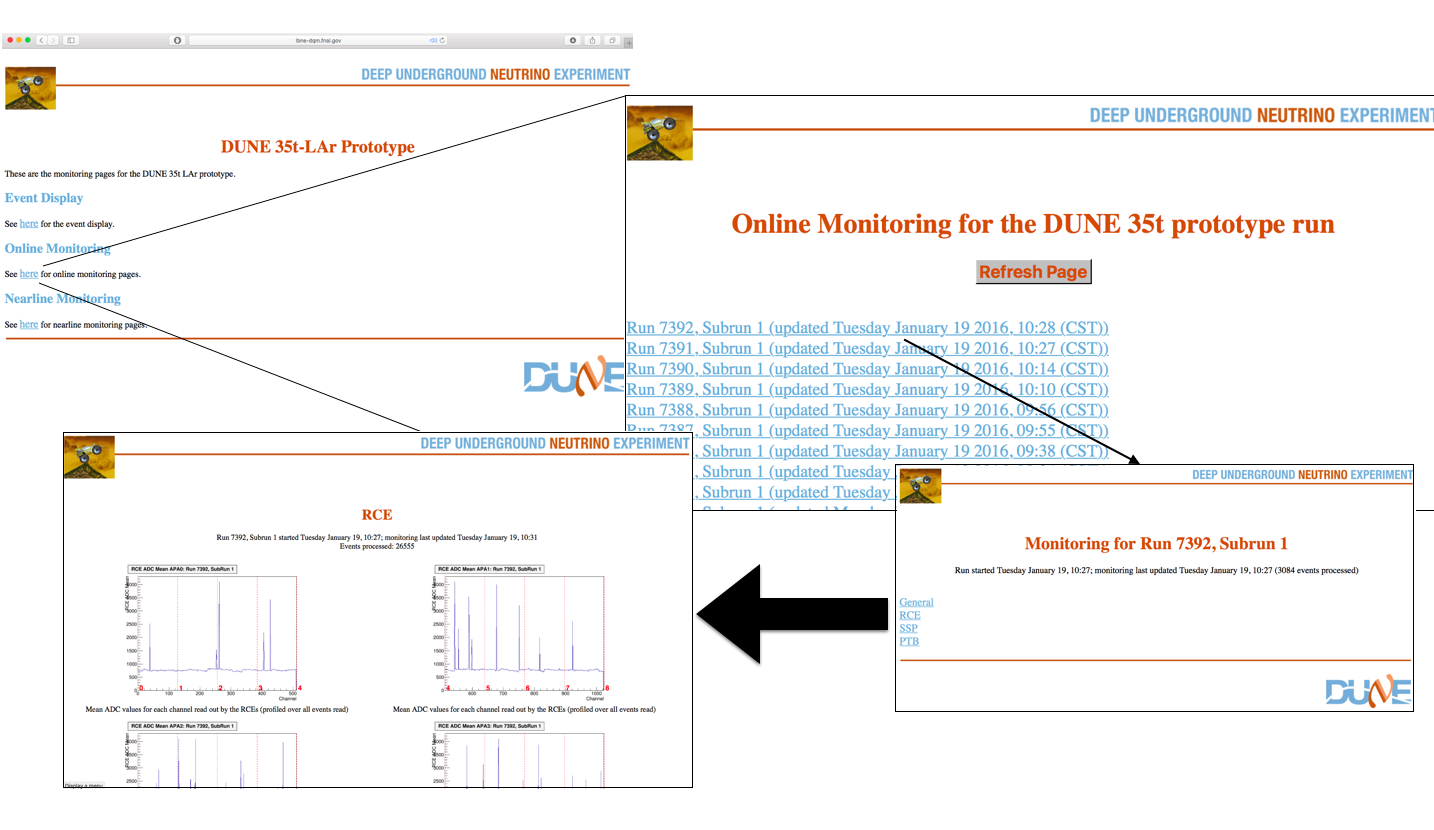
\includegraphics[width=14cm]{webPage.png}
  \caption[Demonstration of the web page developed to display information produced by the online monitoring and event display.]{Demonstration of the web page developed to display information produced by the online monitoring and event display.  The pages are written in HTML and allowed prompt and convenient feedback directly from the DAQ be accessed anywhere and assist in remote monitoring of the experiment.  All previous runs are also kept on the website for reference.}
  \label{fig:WebPage}
\end{figure}

%----------------------------------------------------------------------------------------------------------------------------------------------------------------------------
\section{Online Monitoring Summary}

The monitoring, with web support, was imperative for the success of the 35~ton.  During the ongoing vertical slice tests in summer 2015, the majority of the setup was in place and enabled progress in testing and commissioning the APAs to be completed significantly faster than it otherwise would have been.  During this time, and also during commissioning, the framework was the only way of analysing the data without reading it into LArSoft and writing specific software.  Overall, the framework provided essential feedback and contributed positively towards DAQ uptime during the data taking period.  It is currently in the process of being adapted for future use in DUNE, specifically as part of the ProtoDUNE DAQ for the run in 2018.
